\documentclass[tikz,border=4pt]{standalone}
\usepackage{amsmath,amssymb}
\definecolor{low}{RGB}{31,94,165}\definecolor{dia}{RGB}{214,96,33}\definecolor{up}{RGB}{120,120,128}
% oblique projection: x to the right, y (depth) up and to the right, z up
\newcommand{\block}[6]{% x0, y0, height, colour, top label, side label
  \fill[#4!78!black] (#1+0.9,#2,0) -- (#1+0.9,#2+0.9,0) -- (#1+0.9,#2+0.9,#3) -- (#1+0.9,#2,#3) -- cycle;
  \fill[#4!72!white] (#1,#2,0) -- (#1+0.9,#2,0) -- (#1+0.9,#2,#3) -- (#1,#2,#3) -- cycle;
  \fill[#4!22!white] (#1,#2,#3) -- (#1+0.9,#2,#3) -- (#1+0.9,#2+0.9,#3) -- (#1,#2+0.9,#3) -- cycle;
  \draw[#4!55!black,line width=0.5pt,line join=round]
    (#1,#2,0) -- (#1+0.9,#2,0) -- (#1+0.9,#2+0.9,0) -- (#1+0.9,#2+0.9,#3) -- (#1,#2+0.9,#3) -- (#1,#2,#3) -- cycle
    (#1,#2,#3) -- (#1+0.9,#2,#3) -- (#1+0.9,#2+0.9,#3) (#1+0.9,#2,#3) -- (#1+0.9,#2,0);
  \node[font=\small] at (#1+0.45,#2+0.45,#3) {#5};
  \node[font=\scriptsize,white] at (#1+0.45,#2,#3/2) {#6};
}
\begin{document}
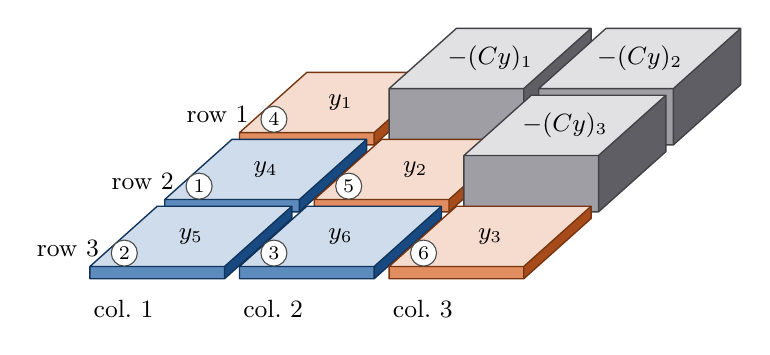
\begin{tikzpicture}[x={(1.9cm,0cm)},y={(0.95cm,0.85cm)},z={(0cm,1.3cm)}]
  % back row: matrix row 1
  \block{0}{2}{0.12}{dia}{$y_1$}{}
  \block{1}{2}{0.55}{up}{$-(Cy)_1$}{}
  \block{2}{2}{0.55}{up}{$-(Cy)_2$}{}
  % middle row: matrix row 2
  \block{0}{1}{0.12}{low}{$y_4$}{}
  \block{1}{1}{0.12}{dia}{$y_2$}{}
  \block{2}{1}{0.55}{up}{$-(Cy)_3$}{}
  % front row: matrix row 3
  \block{0}{0}{0.12}{low}{$y_5$}{}
  \block{1}{0}{0.12}{low}{$y_6$}{}
  \block{2}{0}{0.12}{dia}{$y_3$}{}
  % order in which the columns of C are fixed
  \foreach \x/\y/\k in {0/1/1, 0/0/2, 1/0/3, 0/2/4, 1/1/5, 2/0/6}
    \node[circle,draw=black!70,fill=white,inner sep=1.2pt,font=\scriptsize] at (\x+0.13,\y+0.2,0.12) {\k};
  \node[font=\small,anchor=east] at (-0.1,2.45,0) {row 1};
  \node[font=\small,anchor=east] at (-0.1,1.45,0) {row 2};
  \node[font=\small,anchor=east] at (-0.1,0.45,0) {row 3};
  \node[font=\small] at (0.45,-0.45,0) {col.\ 1};
  \node[font=\small] at (1.45,-0.45,0) {col.\ 2};
  \node[font=\small] at (2.45,-0.45,0) {col.\ 3};
\end{tikzpicture}
\end{document}
